% Gemini theme
% See: https://rev.cs.uchicago.edu/k4rtik/gemini-uccs
% A fork of https://github.com/anishathalye/gemini

\documentclass[final]{beamer}

% ====================
% Packages
% ====================
% \setlength{\paperwidth}{40in}
% \setlength{\paperheight}{30in}

\usepackage[T1]{fontenc}
\usepackage{lmodern}
\usepackage{anyfontsize}
\usepackage[size=custom,width=120,height=80,scale=1.0]{beamerposter}
\usetheme{gemini}
% \usecolortheme{uchicago}
\usecolortheme{stanford}
\usepackage{graphicx}
\usepackage{booktabs}
\usepackage{tikz}
\usepackage{pgfplots}
\usepackage{bbding}
\pgfplotsset{compat=1.17}

% \setlength{\paperwidth}{40in}
% \setlength{\paperheight}{30in}

% ====================
% Lengths
% ====================



% If you have N columns, choose \sepwidth and \colwidth such that
% (N+1)*\sepwidth + N*\colwidth = \paperwidth
\newlength{\sepwidth}
\newlength{\colwidth}
\setlength{\sepwidth}{0.025\paperwidth}
\setlength{\colwidth}{0.3\paperwidth}

\newcommand{\separatorcolumn}{\begin{column}{\sepwidth}\end{column}}


\title{Real-Time Lens Distortion with Deep Learning}


\author{Daniel Huang\inst{1}}

\institute[shortinst]{\inst{1} Institute of Computational and Mathematical Engineering, Stanford}

% ====================
% Footer (optional)
% ====================

\footercontent{
  \href{https://github.com/pi314ever/mathworks-physical-sensor-model}{GitHub: pi314ever/mathworks-physical-sensor-model} \hfill
  ICME Xpo Research Symposium 2023\hfill
  \href{mailto:dhuangpi@alumni.stanford.edu}{dhuangpi@alumni.stanford.edu}
}
% (can be left out to remove footer)

% ====================
% Logo (optional)
% ====================

% use this to include logos on the left and/or right side of the header:
% \logoright{\includegraphics[height=7cm]{logos/cs-logo-maroon.png}}
% \logoleft{\includegraphics[height=7cm]{logos/cs-logo-maroon.png}}

% ====================
% Body
% ====================

\begin{document}

% This adds the Logos on the top left and top right
\addtobeamertemplate{headline}{}
{
  \begin{tikzpicture}[remember picture,overlay]
    \node [anchor=north west, inner sep=3cm] at ([xshift=0.0cm,yshift=1.0cm]current page.north west)
    {
\includegraphics[height=4.0cm]{stanford_logos/icme_logo.png}};
    \node [anchor=north east, inner sep=3cm] at ([xshift=0.0cm,yshift=2.5cm]current page.north east)
    {\includegraphics[height=7.0cm]{stanford_logos/Block_S_2_color.png}};
  \end{tikzpicture}
}

\begin{frame}[t]
  \begin{columns}[t]
    \separatorcolumn

    \begin{column}{\colwidth}

      \begin{block}{Abstract}

        The success of machine learning in recent years relies heavily on high-quality and high-quantity data. For self-driving cars, obtaining real-life data is the best option. However, it is difficult to capture rare but important events and can be costly due to manual labor and traffic disruptions. To address this issue, a simulated environment is used to train AI, where a crucial subsystem is the camera sensor model that translates raw visual data of the physical world to the signals the model “sees”. While simulated environments can generate undistorted images easily using 2D projections, distortions caused by the lens need to be post-processed to account for camera lens properties. Based on the project listed at \cite{mathworks_innovation}, we propose a real-time deep-learning approach for lens distortion correction using a neural network that approximates radial and tangential lens distortion. We present experimental results that can be greatly improved with refinement of model architecture and hyper-parameters.

      \end{block}

      \begin{block}{Background: Terms and Notation}
        \begin{itemize}
          \item \makebox[10cm][l]{\textbf{Radial Distortion}}: Distortion caused by lens' radial symmetry and curvature
          \item \makebox[10cm][l]{\textbf{Tangential Distortion}}: Distortion caused by lens' misalignment with the image plane
          \item \makebox[10cm][l]{\textbf{Distortion Center}}: The point where the optical axis intersects the image plane
          \item \makebox[10cm][l]{$\mathbf{K} = [k_1, k_2, ..., k_i]$}: Radial distortion parameters ($i = 3$ for our model)
          \item \makebox[10cm][l]{$\mathbf{P} = [p_1, p_2, ..., k_j]$}: Tangential distortion parameters ($j = 2$ for our model)
          \item \makebox[10cm][l]{$\mathbf{XY}, (x, y) \in \mathbb{R}_{[-1, 1]}^2$}: Normalized undistorted image coordinates
          \item \makebox[10cm][l]{$\mathbf{XYd}, (x, y) \in \mathbb{R}_{[-1,1]}^2$}: Normalized distorted image coordinates
          \item \makebox[10cm][l]{$\bar{\cdot}\quad$}: Distortion-centered based coordinates
          \item \makebox[10cm][l]{$r^2 = \bar{x}^2 + \bar{y}^2$}: Squared distance from distortion center
        \end{itemize}
      \end{block}

      \begin{block}{Background: Brown's Distortion Model}
        The Brown's distortion model describes radial and tangential lens distortion given calibrated camera parameters using an infinite polynomial series. The radial model is given by:
        \begin{align*}
          x_{d,r} & = x + \bar{x} \left( k_1 r^2 + k_2 r^4 + k_3 r^6 + ... \right) \\
          y_{d,r} & = y + \bar{y} \left( k_1 r^2 + k_2 r^4 + k_3 r^6 + ... \right) \\
        \end{align*}
        And the tangential model is given by:
        \begin{align*}
          x_{d,t} & = x + \left[p_1 (r^2 + 2 \bar{x}^2) + 2 p_2 \bar{x} \bar{y}\right] \left(1 + p_3 r^2 + p_4 r^4 + ...\right) \\
          y_{d,t} & = y + \left[p_2 (r^2 + 2 \bar{y}^2) + 2 p_1 \bar{x} \bar{y}\right]\left(1 + p_3 r^2 + p_4 r^4 + ...\right)
        \end{align*}
        % where $x, y$ are the undistorted coordinates, $x_{d,*}, y_{d,*}$ are the distorted coordinates, $\bar{x}, \bar{y}$ are distortion-centered coordinates, $r^2 = \bar{x}^2 + \bar{y}^2$, $k_i$ are the radial distortion parameters, and $p_i$ are the tangential distortion parameters. \\
        $\Rightarrow$\textbf{Difficulty comes from inverting the distortion model (i.e. solving for $\mathbf{XY}$ given $\mathbf{XYd}$).}
      \end{block}

      \begin{block}{Background: Previous Approaches}

        \textbf{Iterative Approaches} \cite{villiers_centi-pixel_2008}
        \begin{itemize}
          \item Numerically solve for $\mathbf{XY}$ given $\mathbf{XYd}$ using Brown's distortion model using Newton's method or other iterative solvers
          \item Balance between speed and accuracy, is not suitable for real-time applications
        \end{itemize}

        \textbf{Polynomial Approximation of Exact Solutions} \cite{drap_exact_2016}
        \begin{itemize}
          \item Approximate inverse function is possible with an infinite polynomial series
          \item Number of "de-distortion" coefficients required increases dramatically for larger distortions
          \item Not generalizable to cameras with different distortion parameters
        \end{itemize}

      \end{block}

      \begin{block}{Goals and Ideas}
        \textbf{Goals}
        \begin{itemize}
          \item \makebox[7cm][l]{\textit{Real-time}}: Able to distort images accurately
          \item \makebox[7cm][l]{\textit{Generalizable}}: Able to handle different distortion parameters
          \item \makebox[7cm][l]{\textit{Robust}}: Able to handle large distortions
        \end{itemize}

        \textbf{Potential Approaches}
        \begin{itemize}
          \item[$\rightarrow$] \makebox[7cm][l]{\textit{Deep Learning}}: Use a neural network to learn the inverse function
          \item \makebox[7cm][l]{\textit{GANs}}: Use a generative adversarial network to learn the mapping \\
                \makebox[7.25cm][l]{} from undistorted to distorted images
        \end{itemize}
      \end{block}

      % \begin{alertblock}{A highlighted block}

      % \end{alertblock}

    \end{column}

    \separatorcolumn

    \begin{column}{\colwidth}

      \begin{block}{Methodology}
        % TODO: Add algorithm design choices
        \textbf{Model Idea: Point Map Neural Networks (PMNN)}
        \begin{itemize}
          \item[$\star$] \underline{Learn inverse of Brown's distortion function using neural network}
          \item Input: Distorted image coordinates $\mathbf{XYd}$ (what pixels are required to form the distorted image)
          \item Output: Undistorted image coordinates $\mathbf{XY}$ (where to query the pixels from in the original image)
          \item Data: Can generate infinite training examples from Brown's distortion model
        \end{itemize}
        \vspace{-1cm}

        \begin{figure}
          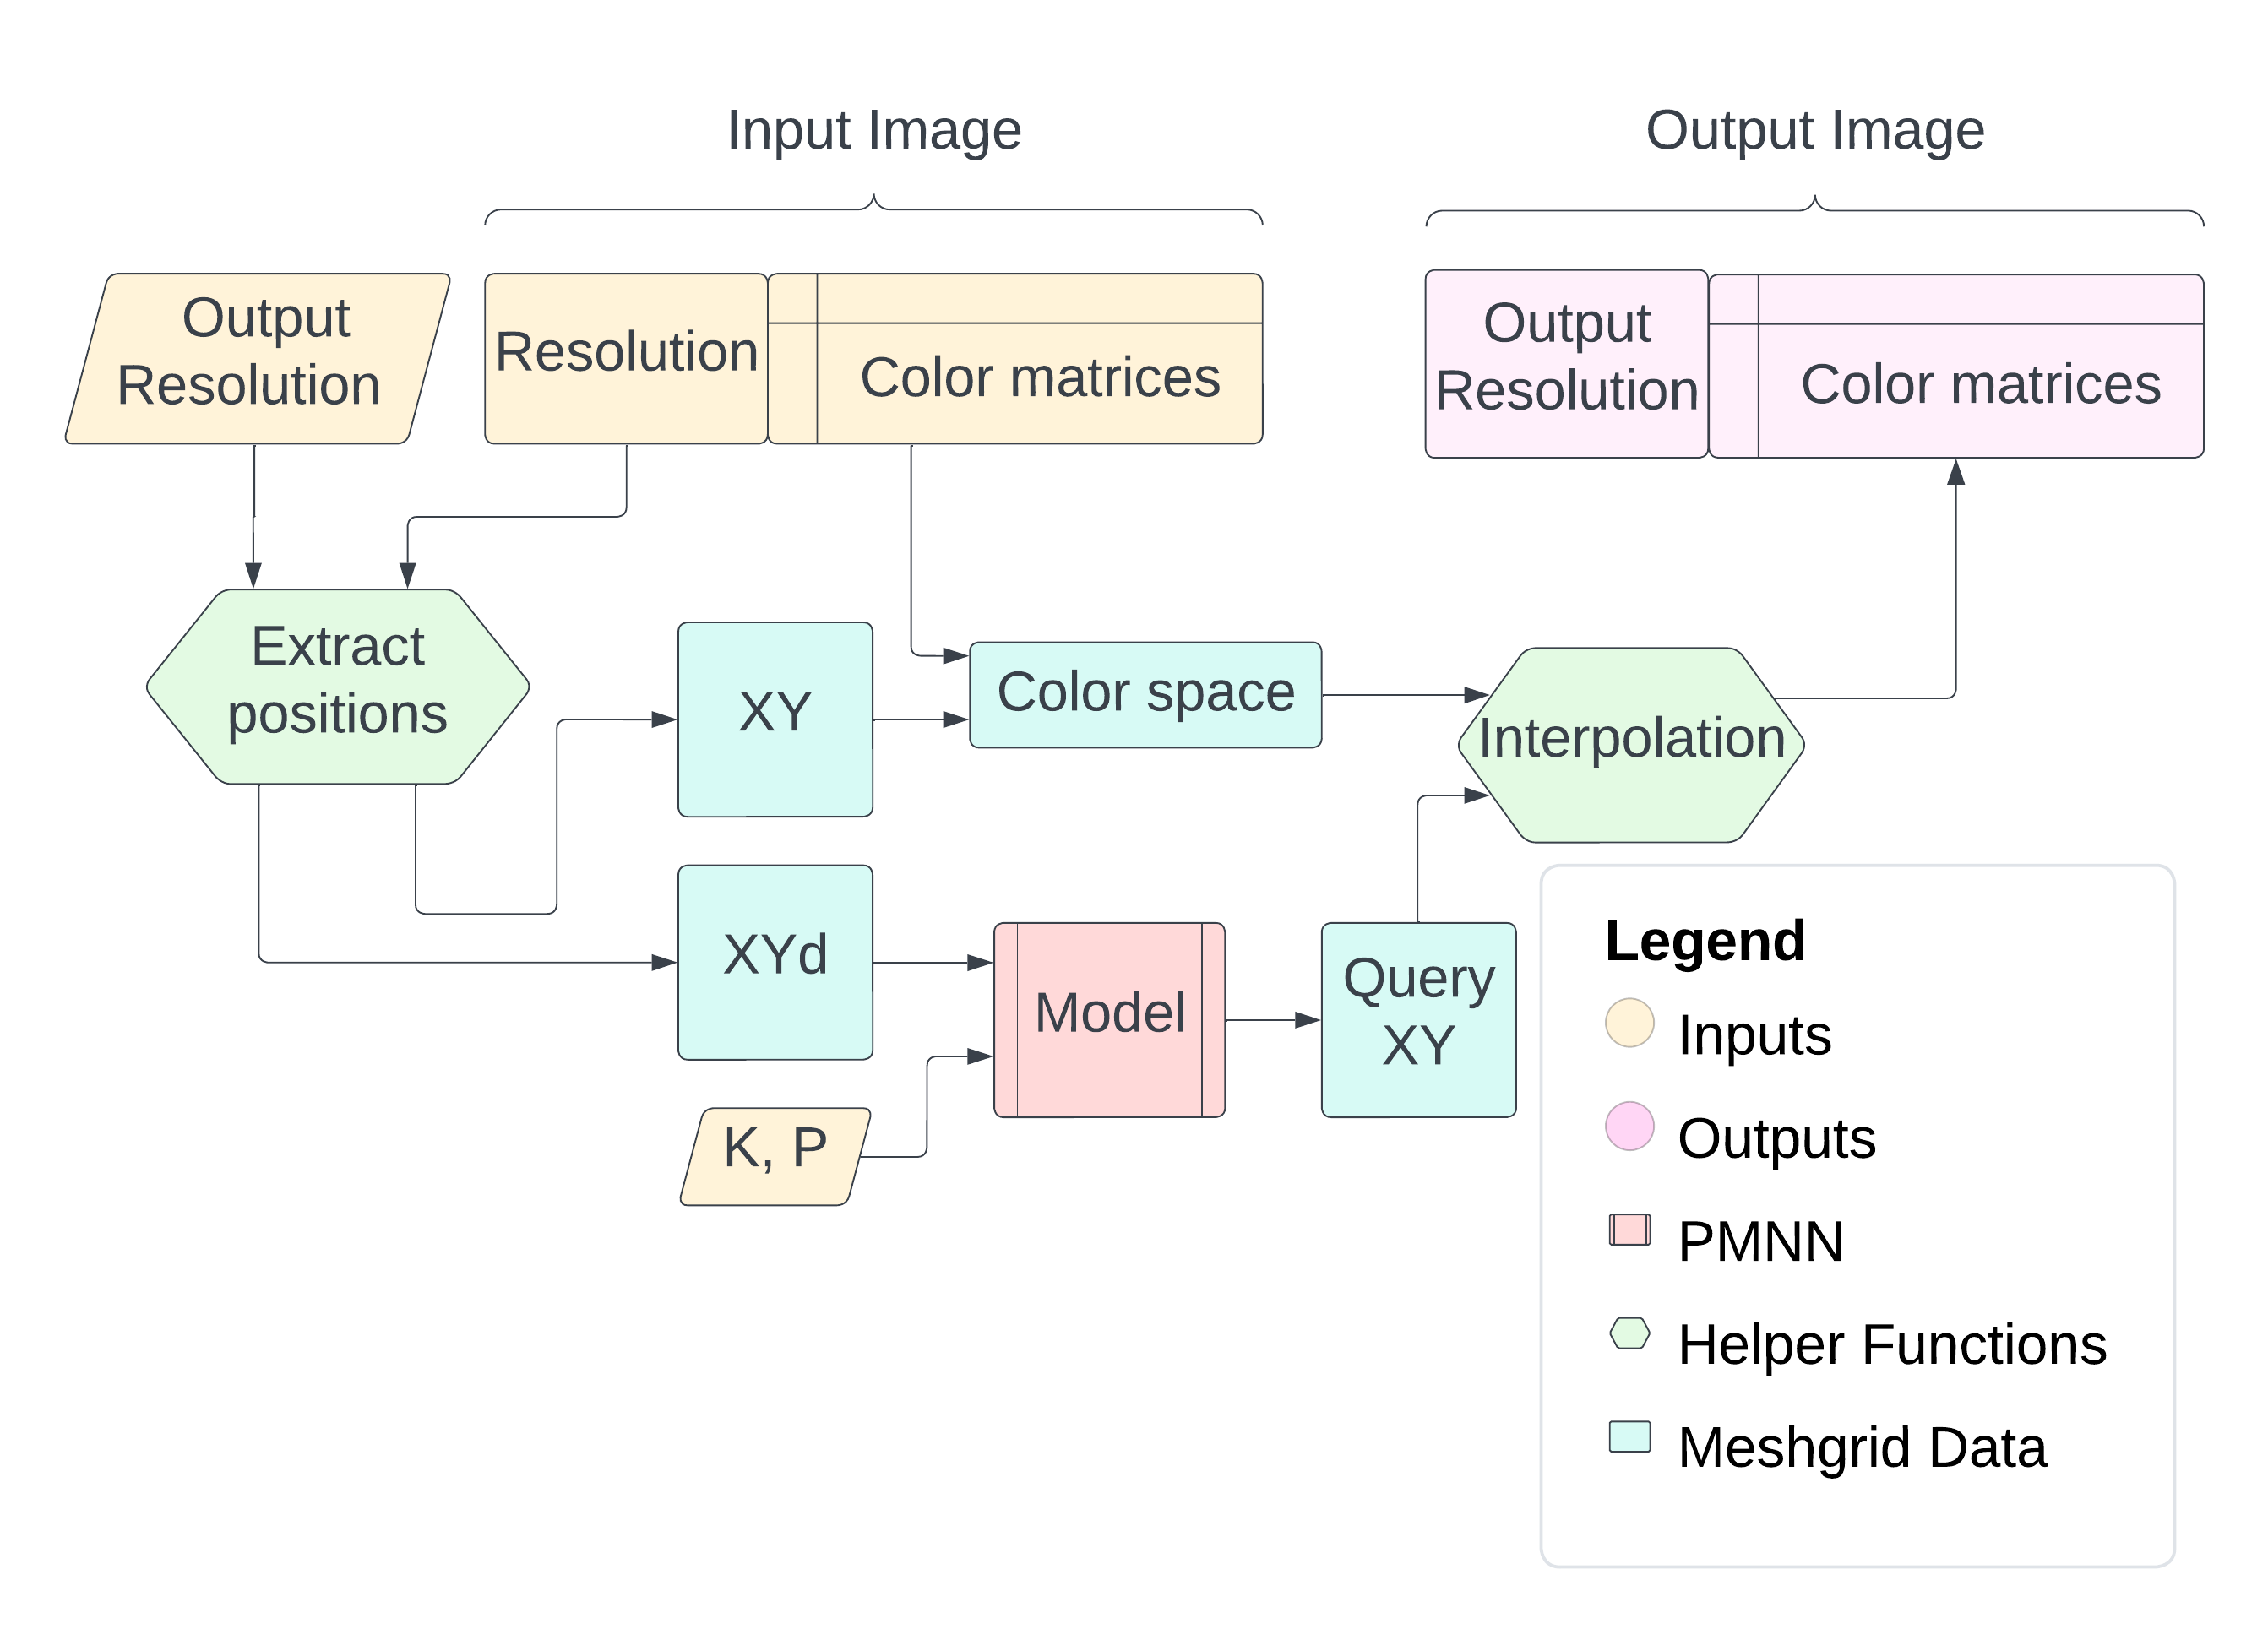
\includegraphics[width=0.90\columnwidth]{images/point_map_diagram.png}
          \caption{Block diagram of image distortion pipeline}
          \label{fig:pipeline}
        \end{figure}

        \textbf{PMNN Architecture}
        \begin{itemize}
          \item \makebox[4cm][l]{\textit{Layers}}: $4 \times 16$ fully connected layers (small) or $6 \times 128$ fully connected layers (large)
          \item \makebox[4cm][l]{\textit{Activation}}: ReLU activation between each layer
          \item \makebox[4cm][l]{\textit{Loss}}: Mean absolute error $\texttt{mean}(|XY - XY_{p}|_1)$ where $|\cdot|_1$ is the 1-norm and $XY_{p}$ is the \\
                \makebox[4.25cm][l]{} predicted undistorted image coordinates
          \item \makebox[4cm][l]{\textit{Optimizer}}: Adam optimizer
          \item \makebox[4cm][l]{\textit{Epochs}}: Trained for 100 epochs, taking best validation loss
          \item \makebox[4cm][l]{\textit{Dataset}}: 2000 random sets of distortions $k_i, p_i \in (-0.1, 0.1)$ with uniformly random chosen\\
                \makebox[4.25cm][l]{}  $XY$ and $XYd$ coordinates. 70\% training, 20\% validation, 10\% test

        \end{itemize}
      \end{block}

      \begin{block}{Experiments}
        \textbf{Radial Distortion $K = (0.1, 0.03, 0.005)$}\\
        \textbf{Ground Truth}: Gradient Descent on $XYd - \texttt{distort}(XY)$, where $\texttt{distort}(XY)$ distorts the image using Brown's distortion model
        % \begin{figure}
        %   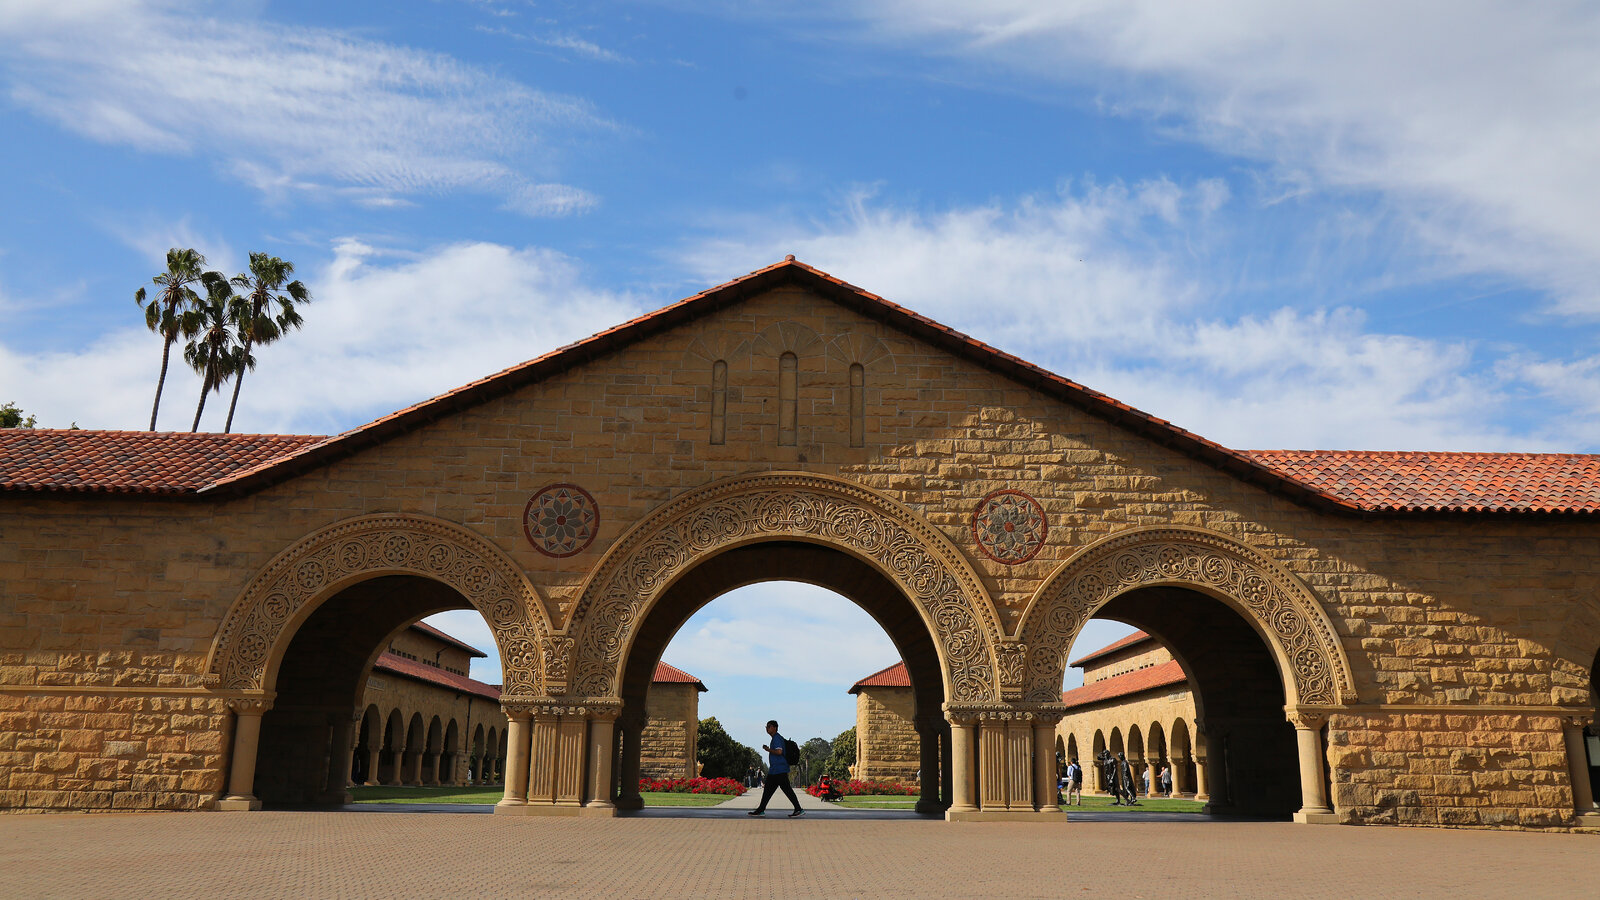
\includegraphics[width=0.48\columnwidth]{images/stanford.png}
        %   
\includegraphics[width=0.48\columnwidth]{images/checkerboard.jpg}
        %   \caption{Stanford Main Quad and checkerboard images used for benchmarking distortions}
        % \end{figure}
        \begin{figure}
          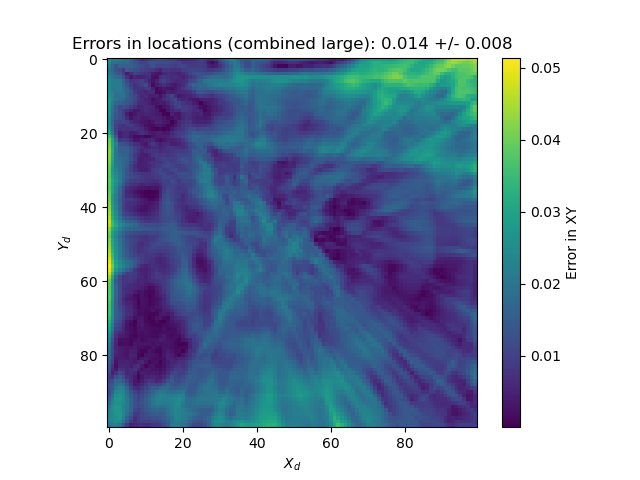
\includegraphics[width=0.45\columnwidth]{images/combined_large_error_heatmap.png}
          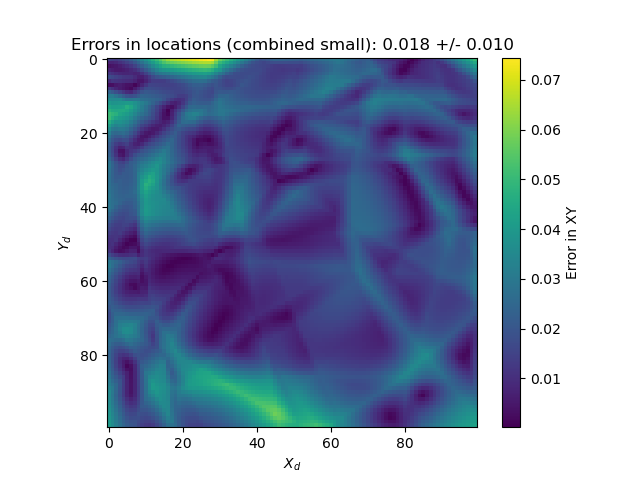
\includegraphics[width=0.45\columnwidth]{images/combined_small_error_heatmap.png}
          \caption{Heatmaps of error between ground truth and PMNN undistorted coordinates for large (left) and small (right) models}
        \end{figure}
      \end{block}

    \end{column}

    \separatorcolumn

    \begin{column}{\colwidth}
      \begin{block}{Experiments (cont.)}
        \begin{figure}
          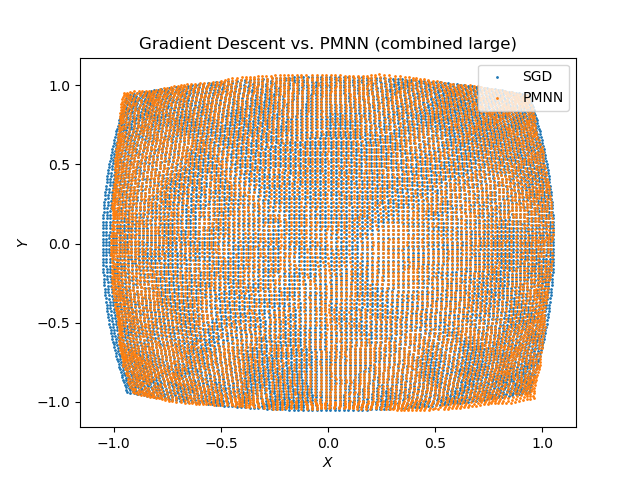
\includegraphics[width=0.48\columnwidth]{images/combined_large_pointmap.png}
          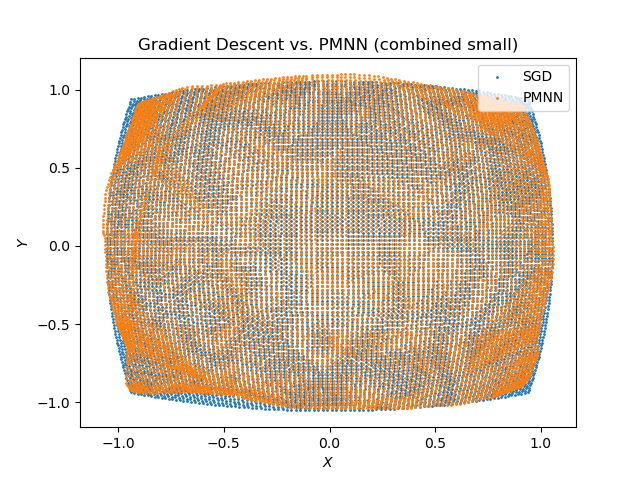
\includegraphics[width=0.48\columnwidth]{images/combined_small_pointmap.png}
          \caption{Point map comparison between ground truth and PMNN undistorted coordinates for large (left) and small (right) models}
        \end{figure}

        \begin{figure}
          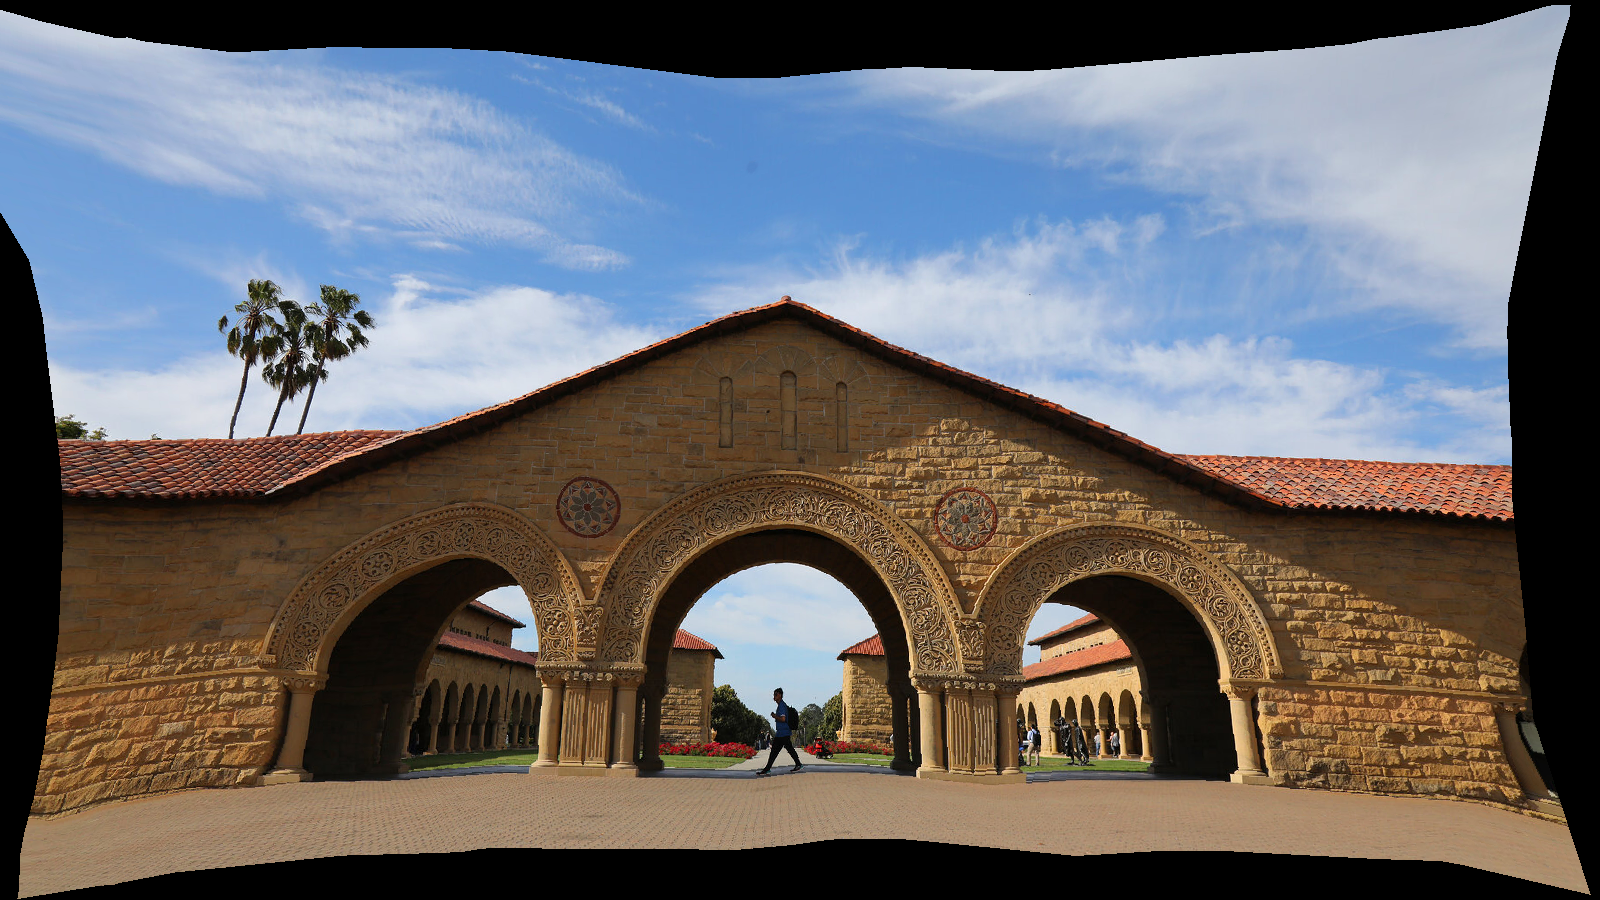
\includegraphics[width=0.48\columnwidth]{images/combined_stanford.png}
          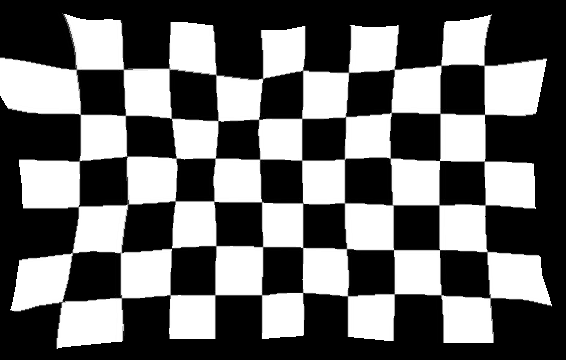
\includegraphics[width=0.44\columnwidth]{images/combined_checkerboard.png}
          \caption{Stanford Main Quad and checkerboard images distorted using the small model}
        \end{figure}
      \end{block}

      \begin{block}{Results and Discussion}
        \begin{itemize}
          \item Neither model is capable of creating visually-consistent distortions (many artifacts)
          \item Large model slightly more accurate, but edges are problematic
          \item Much faster than gradient descent ($\approx$70 ms for PMNN on one core vs 17+ seconds for GD on multiple cores)
          \item Errors may come from inconsistencies between training data and expected usage
        \end{itemize}

        \textbf{Future Work}
        \begin{itemize}
          \item \makebox[10cm][l]{\textbf{Model Improvements}}: Rapid post-processing to reduce noise in output
          \item \makebox[10cm][l]{\textbf{Iterative Models}}: Design model with iterative refinement to improve accuracy \cite{andrychowicz_learning_2016}
        \end{itemize}

      \end{block}

      \begin{block}{Acknowledgements}
        \begin{itemize}
          \item \makebox[7cm][l]{\textbf{Industry Mentor}}: Reza Fazel-Rezai, Ph.D., P.Eng., MathWorks
          \item \makebox[7cm][l]{\textbf{Faculty Mentor}}: Alan Gous, Ph.D.
          \item \makebox[7cm][l]{\textbf{Xplore Mentor}}: Kari Hanson
        \end{itemize}
      \end{block}

      \begin{block}{References}

        \nocite{*}
        \footnotesize{\bibliographystyle{plain}\bibliography{poster}}

      \end{block}

    \end{column}

    \separatorcolumn
  \end{columns}
\end{frame}

\end{document}
